\documentclass[8pt]{beamer}

\usepackage{listings}

\definecolor{codegreen}{rgb}{0,0.6,0}
\definecolor{codegray}{rgb}{0.5,0.5,0.5}
\definecolor{codepurple}{rgb}{0.58,0,0.82}
\definecolor{backcolour}{rgb}{0.95,0.95,0.92}

\lstdefinestyle{mystyle}{
backgroundcolor=\color{backcolour},
commentstyle=\color{codegreen},
keywordstyle=\color{magenta},
numberstyle=\tiny\color{codegray},
stringstyle=\color{codepurple},
basicstyle=\ttfamily\small,
breakatwhitespace=false,
breaklines=true,
captionpos=b,
keepspaces=true,
numbers=left,
numbersep=5pt,
showspaces=false,
showstringspaces=false,
showtabs=false,
tabsize=2
}

\usetheme[sectionpage=none]{metropolis}
\setbeamertemplate{section in toc}[sections numbered]

\title{Library development}
\author{Julien Schueller - Phimeca}
\date{March 28th-31th 2023}
\titlegraphic{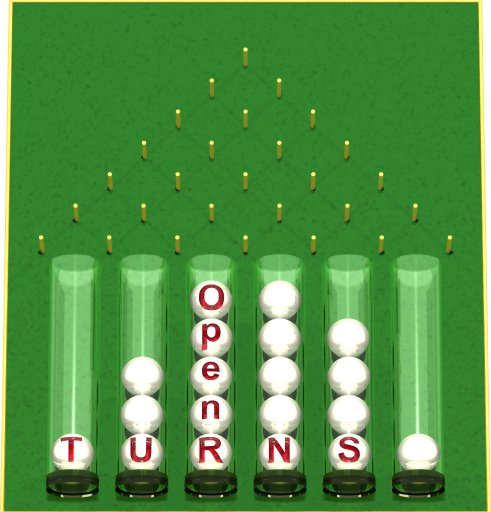
\includegraphics[height=1.5cm]{logoOT}}
\institute{\small OpenTURNS Consortium}


\begin{document}

\frame{\titlepage}

% necessaire pour la table des matieres
\part{Main part}

% table des matieres
\begin{frame}
  \frametitle{CMake compilation infrastructure}
  \tableofcontents[part=1]
\end{frame}
%%%%%%%%%%%%%%%%%%%%%%%%% 
% The OpenTURNS package %
%%%%%%%%%%%%%%%%%%%%%%%%% 

\section[CMake]{CMake}
%%%%%%%%%%%%% 
% The tools %
%%%%%%%%%%%%% 
\begin{frame}
  \frametitle{CMake}
  \begin{block}{Basics}

  CMake is an extensible, open-source system that manages the build process in an operating system and in a compiler-independent manner and covers:
  
\begin{itemize}
  \item The detection and configuration aspects of the platform;

  \item The dependency management of the sources;

  \item The generation of parallel makefiles;

  \item The regression tests.
\end{itemize}

Some core ideas of CMake:
\begin{itemize}
  \item All the configuration is done through a hierarchy of text files written in the CMake macro language.
  
  \item Unlike many cross-platform systems, CMake is designed to be used in conjunction with several generation tools.
  (Make, NMake, Ninja, ...)
\end{itemize}

  \end{block}
\end{frame}

\begin{frame}
  \frametitle{The CMake compilation infrastructure}
  \begin{block}{CMake}
    It consists configuration files placed in each source directory (called CMakeLists.txt files) and cover:
    \begin{itemize}
    \item \emph{configuration} through a master configuration file: the top-level CMakeLists.txt file;
    \item \emph{source organization} through a set of CMakeLists.txt files disseminated in the whole source tree: each
    \item \emph{dependency detection} through a set of detection macros: the several .cmake files;
        such file includes the declaration of the several source files and associated header files, and make a recursive call to the subdirectories.
    \item \emph{testing} using the associated CTest testing utility, responsible for running C++ and Python tests.
    \end{itemize}
  \end{block}
\end{frame}

\begin{frame}[fragile]
  \frametitle{CMake usage}

  \lstset{style=mystyle}
  
\begin{lstlisting}
mkdir build && cd build
cmake -DCMAKE_BUILD_TYPE=RelWithDebInfo
  -DCMAKE_INSTALL_PREFIX=$PWD/install
  -DCMAKE_CXX_FLAGS="-Wall -Wextra -D_GLIBCXX_ASSERTIONS"
  -DSWIG_COMPILE_FLAGS="-O1"
  -DUSE_SPHINX=OFF -DSPHINX_FLAGS="-W -T -j4"
  ..

make install -j4
ctest -R pyinstall -j4

make tests -j4
ctest -R cppcheck -j4
\end{lstlisting}

\end{frame}

%%%%%%%%%%%%%%%%%% 
% Development process
%%%%%%%%%%%%%%%%%% 
\section[C++ development process]{C++ development process}
\begin{frame}
  \frametitle{C++ development process}
  \begin{block}{Two main situations}
    There are two distinct situations in the development of additional capabilities of OpenTURNS:
    \begin{itemize}
      \item The addition of a new instance of an existing concept;
      \item The introduction of a new concept.
    \end{itemize}
    The associated development process shares the same principles in both cases, but the details are more involved in the second case.\\
    Both cases are covered in the \alert{Developer} documentation that comes with OpenTURNS, only the first situation will be covered here. We suppose that our extension consist in the creation of a new class called MyClass in an existing directory.
  \end{block}
\end{frame}
%%%%%%%%%%%%%%%%%%% 
% Add a new class
%%%%%%%%%%%%%%%%%%% 
\begin{frame}[fragile]
  \frametitle{Populate an existing concept}
  \begin{block}{Step 1: create the header file and the associated source file}
    Create MyClass.cxx and openturns/MyClass.hxx in a subdirectory of lib/src. The files must have the standard header,
    with a brief description of the class using the Doxygen format and the standard reference to the LGPL license.
  
  For the header file MyClass.hxx, the interface must be embraced between the preprocessing clauses to prevent from multiple inclusions.

\begin{lstlisting}
#ifndef OPENTURNS_MYCLASS_HXX
#define OPENTURNS_MYCLASS_HXX

class OT_API MyClass {...};

#endif /* OPENTURNS_MYCLASS_HXX */
\end{lstlisting}

  See any pair of .hxx/.cxx files in the current directory and the coding section as a guide for your development: the use of namespaces, case convention for the static methods, the other methods and the attributes, the trailing underscore for the attribute names to name a few rules.
  \end{block}
\end{frame}
%%%%%%%%%%%%%%%%%% 
% Add a new class
%%%%%%%%%%%%%%%%%% 
\begin{frame}
  \frametitle{Populate an existing concept}
  \begin{block}{Step 2: update the CMake source configuration}
    Modify the CMakeList.txt file in some lib/src subdirectory:
    \begin{itemize}
    \item add openturns/MyClass.hxx using the instruction {\ttfamily ot\_install\_header\_file (MyClass.hxx)}
    \item add MyClass.cxx using the instruction {\ttfamily ot\_add\_source\_file (MyClass.cxx)}
    \end{itemize}
    At this point you can build the library with the new class:\\
     {\ttfamily make}
  \end{block}
\end{frame}
%%%%%%%%%%%%%%%%%% 
% Add a new class
%%%%%%%%%%%%%%%%%% 
\begin{frame}
  \frametitle{Populate an existing concept}
  \begin{block}{Step 2b: update the subdirectory header}
    Modify the OTsubdir.hxx file in lib/src/subdir/openturns/ to include the new header:\\
    {\ttfamily \#include "openturns/MyClass.hxx"}

  \end{block}
\end{frame}
%%%%%%%%%%%%%%%%%%
% Add a new class
%%%%%%%%%%%%%%%%%% 
\begin{frame}
  \frametitle{Populate an existing concept}
  \begin{block}{Step 3: the source code of the test(s)}
    Create a test file t\_MyClass\_std.cxx in the directory lib/test. This test file must check at least the standard functionalities of the class MyClass. If relevant, some specific aspects of the class can be checked in specific other test files, such as the exceptional behaviour of the class or its functionalities in extrem configurations (large data set, hard to solve problems etc.).
  \end{block}
\end{frame}

\begin{frame}[fragile]
  \frametitle{Populate an existing concept}
%   \begin{block}{Step 3: the source code of the test(s)}
  \lstset{style=mystyle}
  
\begin{lstlisting}
int main(int, char *[])
{
  try
  {
    ...
    MyClass algorithm(problem);
    algo.run();
    OptimizationResult result = algo.getResult();
    Point x_star = result.getOptimalPoint();
    Point p_ref = {0.6, 8.9};
    std::cout << "x_star=" << x_star << std::endl;
    assert_almost_equal(x_star, p_ref);
  }
  catch (TestFailed & ex)
  {
    std::cerr << ex << std::endl;
    return ExitCode::Error;
  }
  return ExitCode::Success;
}
\end{lstlisting}
\end{frame}

%%%%%%%%%%%%%%%%%%
% Add a new class
%%%%%%%%%%%%%%%%%% 
\begin{frame}[fragile]
  \frametitle{Populate an existing concept}
  \begin{block}{Step 4: update the CMake test configuration}
    Modify the CMakeList.txt file in the lib/test directory:\\
\begin{lstlisting}
ot_check_test (MyClass_std)
\end{lstlisting}
    At this point you can build the specific test:\\
\begin{lstlisting}
make t_MyClass_std
\end{lstlisting}
     And run it:\\
\begin{lstlisting}
./lib/test/t_MyClass_std
\end{lstlisting}
  \end{block}
  
\end{frame}
%%%%%%%%%%%%%%%%%%
% Add a new class
%%%%%%%%%%%%%%%%%% 
\begin{frame}[fragile]
  \frametitle{Populate an existing concept}
  \begin{block}{Step 5: update the CMake file of the lib/test directory}
    If necessary an expected test result named t\_MyClass\_std.expout:\\
\begin{lstlisting}
./lib/test/t_MyClass_std > ../lib/test/t_MyClass_std.expout
\end{lstlisting}

    The content of this file is compared to the output of the cxx test executable when tests are run.

    At this point you can run the specific test:\\
\begin{lstlisting}
ctest -R cppcheck_MyClass_std --output-on-failure
\end{lstlisting}
  \end{block}
\end{frame}

%%%%%%%%%%%%%%%%%%
% Add a new class
%%%%%%%%%%%%%%%%%% 
\begin{frame}
  \frametitle{Populate an existing concept}
  \begin{block}{Step 7: validation}
    If the validation of your class involved advanced mathematics, or was a significant work using other tools, you can add this validation in the validation/src directory.

  \end{block}
\end{frame}
%%%%%%%%%%%%%%%%%%
% Critical points
%%%%%%%%%%%%%%%%%% 
\begin{frame}
  \frametitle{Tips and tricks}
  \begin{block}{Critical points}
    \begin{itemize}
    \item All the classes must include the {\ttfamily CLASSNAME} macro (defined in Base/Common/Object.hxx) in their header file in order to benefit from the (basic) introspection mechanisms. The associated {\ttfamily CLASSNAMEINIT} macro must be used in the corresponding source file.
    \item All the class corresponding to persistent objects must instantiate a static parameterized factory in their source file.
        \item All the classes must include the {\ttfamily OT\_API} macro in their header file in order to export their symbols for win32 targets.
    \item Implementation classes must provide a clone method.
      \item Use std::copy to duplicate chunks of contiguous data
    \end{itemize}
  \end{block}
\end{frame}

%%%%%%%%%%%%%%%%%%
% Critical points
%%%%%%%%%%%%%%%%%% 
\begin{frame}
  \frametitle{Tips and tricks}
  \begin{block}{Critical points}
    \begin{itemize}
      \item The const correctness of the code is very important, both for the signature of the methods and for the temporary variables.
      \item Simple types must use OpenTURNS typedefs (Bool, UnsignedInteger, Scalar, Complex)
      \item Simple types attributes must be initialized in constructors (or in the header itself).
      \item All the object arguments must be passed using const references. The use of non const references to make side effects must be limited as much as possible.
      \item Most of the coding rules are described in the coding rules section, but you can infer the rules by looking at the existing code. \alert{The key point is that the only difficult points should be the conception and the algorithms, not the indentation or the coding style!}
    \end{itemize}
  \end{block}
\end{frame}

%%%%%%%%%%%%%%%%%%
% Critical points
%%%%%%%%%%%%%%%%%% 
\begin{frame}
  \frametitle{Development of a new distribution}
  \begin{block}{Practical case: adding a new distribution to the C++ library}
    \begin{itemize}
    \item From an algorithmic point of view, the minimum to do is to implement the {\ttfamily Scalar computeCDF(const Point \& point)} method.
    \item From a development process point of view, each trainee is expected to go through at least the 6 first steps.
    \item The other methods should be added in the following order:
      \begin{enumerate}
      \item {\ttfamily Scalar computePDF(const Point \& point)}
      \item {\ttfamily Point getRealization()}
      \item {\ttfamily Scalar computeScalarQuantile(const Scalar prob, const Bool tail, const Scalar precision)}
      \item {\ttfamily void computeMean() const}
      \item {\ttfamily void computeCovariance() const}
      \end{enumerate}
    \end{itemize}
  \end{block}
\end{frame}


% table des matieres
\begin{frame}
  \frametitle{SWIG}
  \tableofcontents[part=1]
\end{frame}
%%%%%%%%%%%%%%%%%%%%%%%%% 
% The OpenTURNS package %
%%%%%%%%%%%%%%%%%%%%%%%%% 
\section[SWIG]{SWIG}
%%%%%%%%%%%%%
% The tools %
%%%%%%%%%%%%%
\begin{frame}
  \frametitle{OpenTURNS Python bindings}
  \begin{block}{A user-friendly interface for the OpenTURNS library}
    OpenTURNS is intended to be used for complex industrial application. It means the ability to pilot complex simulation software, but also complex probabilistic modelling and involved strategies for uncertainty propagation. A typical graphical user interface does not provide the flexibility to address such needs, so OpenTURNS is proposed to the user as a Python module.\\
    Python is a full-featured object oriented programming language, and allows for complex scripting of functionalities coming from numerous modules. A typical uncertainty propagation study can be fully implemented using OpenTURNS only, but it can be easier to delegate some treatments to other graphical, statistical or numerical packages. For complex studies, it is the only way to do the job.\\
    The standard extension mechanisms proposed by Python to bind an external library are very low level mechanisms. It is mainly a C interface through which all the types are lost: the arguments are mainly {\ttfamily void *} pointers, and a lot of transtyping is required in order to make the things work.\\
    Several higher level tools have been developed in order to ease this binding, one of the most advanced being SWIG.
  \end{block}
\end{frame}

\begin{frame}
  \frametitle{SWIG: Simplified Wrapper and Interface Generator}
  \begin{block}{A tool to link C/C++ library with script languages}
    SWIG is a software development tool that connects programs written in C and C++ with a variety of high-level programming languages. SWIG is used with different types of target languages including common scripting languages such as Perl, PHP, Python, Tcl and Ruby. The list of supported languages also includes non-scripting languages such as C\#, Common Lisp (CLISP, Allegro CL, CFFI, UFFI), D, Go language, Java, Lua, Modula-3, OCAML, Octave and R. Also several interpreted and compiled Scheme implementations (Guile, MzScheme/Racket, Chicken) are supported. SWIG is most commonly used to create high-level interpreted or compiled programming environments, user interfaces, and as a tool for testing and prototyping C/C++ software. SWIG is typically used to parse C/C++ interfaces and generate the 'glue code' required for the above target languages to call into the C/C++ code.
  \end{block}
\end{frame}

\begin{frame}
  \frametitle{SWIG: Simplified Wrapper and Interface Generator}
  \begin{block}{A tool to link C/C++ library with script languages}
  SWIG needs a set of interface files (.i) with custom glue code.
  
    SWIG parses the library headers and swig interface files to
  generates the corresponding module source yet to be compiled to
  produce a binary python module, see.\\
  The process is split between several modules for modularity and to speed up compilation
  time with parallel builds.
  \end{block}
  \centering \resizebox{!}{4cm}{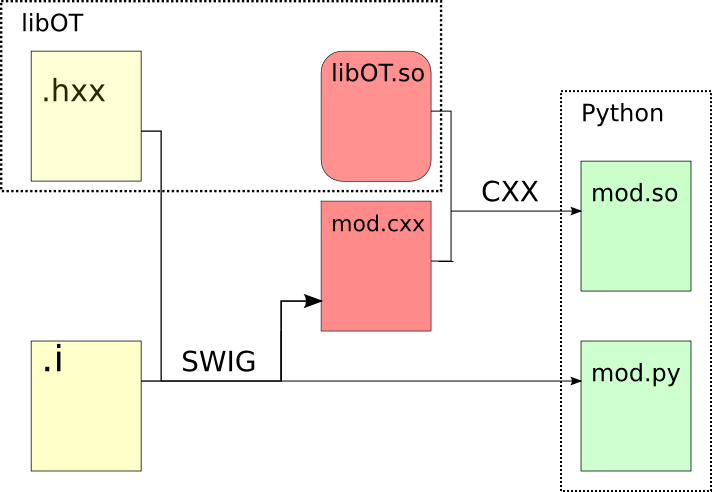
\includegraphics{swig.png}}
\end{frame}


\section[Python development process]{Python development process}
%%%%%%%%%%%%%%%%%% 
% Add a new class
%%%%%%%%%%%%%%%%%% 
\begin{frame}[fragile]
  \frametitle{Integration of the new class in the Python bindings}
  \begin{block}{Step 9: create the SWIG interface file}
    In order to make the new class visible in the OpenTURNS Python module, you have to create a specific SWIG interface file, namely the file MyClass.i in the python/src directory. In most situations, it should be as simple as:
    \small

    \begin{lstlisting}
// SWIG file MyClass.i

%{
#include "MyClass.hxx"
%}

%include MyClass.hxx

namespace OT {
%extend MyClass {

MyClass(const MyClass & other) {
  return new OT::MyClass(other);
}

}}
\end{lstlisting}
    
    \normalsize
  \end{block}
\end{frame}
%%%%%%%%%%%%%%%%%% 
% Add a new class
%%%%%%%%%%%%%%%%%% 
\begin{frame}
  \frametitle{Integration of the new class in the Python bindings}
  \begin{block}{Step 10: integrate the SWIG interface file into the whole Python interface}
    \begin{itemize}
    \item Locate in which of the Python submodule SWIG file you have to include MyClass.i (look for classes from the same source subdirectory) 
    \item Add MyClass.i in the SWIG module source python/src/xxx\_module.i
    \item Modify the CMakeLists file in python/src: add MyClass.i to the identified SWIG module
    \end{itemize}
  \end{block}
\end{frame}
%%%%%%%%%%%%%%%%%% 
% Add a new class
%%%%%%%%%%%%%%%%%% 
\begin{frame}[fragile]
  \frametitle{Integration of the new class in the Python bindings}
  \begin{block}{Step 11: test the new class in the Python module}
    \begin{itemize}
    \item Create a test file t\_MyClass\_std.py in the directory python/test. This test implements the same tests than t\_MyClass\_std.cxx, but using Python.
\begin{lstlisting}
...
algo = ot.MyClass(problem)
algo.run()
result = algo.getResult()
p_ref = [0.6, 8.9]
x_star = result.getOptimalPoint()
ott.assert_almost_equal(x_star, p_ref)
\end{lstlisting}
        
    \item If necessary, create an expected result file t\_MyClass\_std.expout for the python test.
    \item Modify the CMakeLists file in python/test:
\begin{lstlisting}
ot_pyinstallcheck_test (MyClass_std IGNOREOUT)
\end{lstlisting}

\item At this point you can run the specific test:\\
\begin{lstlisting}
ctest -R pyinstallcheck_MyClass_std --output-on-failure
\end{lstlisting}

    \end{itemize}
  \end{block}
\end{frame}
%%%%%%%%%%%%%%%%%% 
% Add a new class
%%%%%%%%%%%%%%%%%% 
\begin{frame}[containsverbatim]
  \frametitle{Integration of the new class in the Python bindings}
  \begin{block}{Step 12: write the docstring documention}
    \begin{itemize}
    \item Create a docstring file python/src/MyClass\_doc.i.in:
    
    This file contains the documentation of new methods following the Numpydoc style:

    \begin{lstlisting}
%feature("docstring") OT::MyClass
"MyClass optimization solver.

Parameters
----------
problem : :class:`~openturns.OptimizationProblem`
    Optimization problem to solve
p1 : int
    Awesome parameter."
\end{lstlisting}

\item Make sure it will be included from MyClass.i:\\
\begin{lstlisting}
%include MyClass_doc.i
\end{lstlisting}
\end{itemize}
  \end{block}
\end{frame}
%%%%%%%%%%%%%%%%%% 
% Add a new class
%%%%%%%%%%%%%%%%%% 
\begin{frame}[containsverbatim]
  \frametitle{Integration of the new class in the Python bindings}
  \begin{block}{Step 13: add an entry in the API manual}
    \begin{itemize}
    \item Find the right .rst in python/doc/user\_manual;
    \item Add an entry in the restructured text format:
    \end{itemize}
  \end{block}
\end{frame}
%%%%%%%%%%%%%%%%%% 
% Add a new class
%%%%%%%%%%%%%%%%%% 
\begin{frame}[containsverbatim]
  \frametitle{Integration of the new class in the Python bindings}
  \begin{block}{Step 14: update the examples manual}    
    \begin{itemize}
    \item Add or expand a \texttt{plot\_xxx.py} script in a \texttt{python/doc/examples} subdirectory
    \end{itemize}
  \end{block}
\end{frame}
%%%%%%%%%%%%%%%%%% 
% Add a new class
%%%%%%%%%%%%%%%%%% 
\begin{frame}
  \frametitle{Integration of the new class in the Python bindings}
  \begin{block}{Pitfalls, tips and tricks}
    Python does not support nested classes. As such, SWIG does  not propose any automatic mechanism to expose such classes in Python. The solution retained in OpenTURNS is to typedef the instantiations of the parametric classes to explicit new classes. Example:
    \begin{itemize}
    \item In the C++ library:
      \small
      \begin{tabular}{l}
        \ttfamily template <class T> class Collection \\
        \ttfamily typedef Collection< Distribution > DistributionCollection;
      \end{tabular}
      \normalsize
    \item In the SWIG interface file:
      \small
      \begin{tabular}{l}
        \ttfamily \% template(DistributionCollection) OT::\\
        \ttfamily Collection<OT::Distribution>;
      \end{tabular}
      \normalsize
    \end{itemize}
    For the nested classes, no reasonable solution has been found: we had to unnest the class in the SWIG interface file, creating C++ source code to be maintained in the SWIG interface. We decided to do this job in the C++ library instead.
  \end{block}
\end{frame}
%%%%%%%%%%%%%%%%%% 
% Add a new class
%%%%%%%%%%%%%%%%%% 
\begin{frame}
  \frametitle{Integration of the new class in the Python bindings}
  \begin{block}{Automatic conversion between C++ types into Python types}
    The automatic conversion of types is needed both to ease the writing of OpenTURNS scripts by Python users. Two distinct cases are of concern with OpenTURNS:
    \begin{itemize}
    \item The automatic conversion between Python lists/arrays and OpenTURNS collections;
    \item The automatic promotion of implementation classes into interface classes.
    \end{itemize}
    The first point is addressed both at the Python level and the C++ level:
    \begin{itemize}
    \item A set of parametric wrapping methods are defined in a C++ header (see PythonWrappingFunction.hxx in python/src);
    \item All the parametric classes are extended at the SWIG level with constructors from Python objects, using these wrapping methods.
    \end{itemize}
    The second point is due to the lack of capabilities of SWIG to identify correctly the Bridge pattern and use the existing constructors in order to perform the automatic conversions. It results in a need to make these conversions explicitly in the Python scripts, which is not natural for a Python programmer. The solution retained in OpenTURNS is to use the {\ttfamily typemap} service of SWIG and the wrapping methods in order to make these conversions automatic for the Python programmer (see Distribution.i in python/src).
  \end{block}
\end{frame}

\end{document}
